\chapter{Fundamentos teóricos matemáticos.}
\section{Cálculo vectorial.}\label{sec:Calculo vectorial.}
\setcounter{equation}{0}
\setcounter{figure}{0}

La palabra vector significa 'que conduce', fisicamente hablando es un elemento que posee magnitud, dirección y sentido. Siendo la magnitud la longitud del vector, la dirección la oriendación de la flecha, el sentido indica hacia el lado donde se dirige el vector.  Su expresión geométrica es la de una recta.
\begin{figure}[H]
\centering
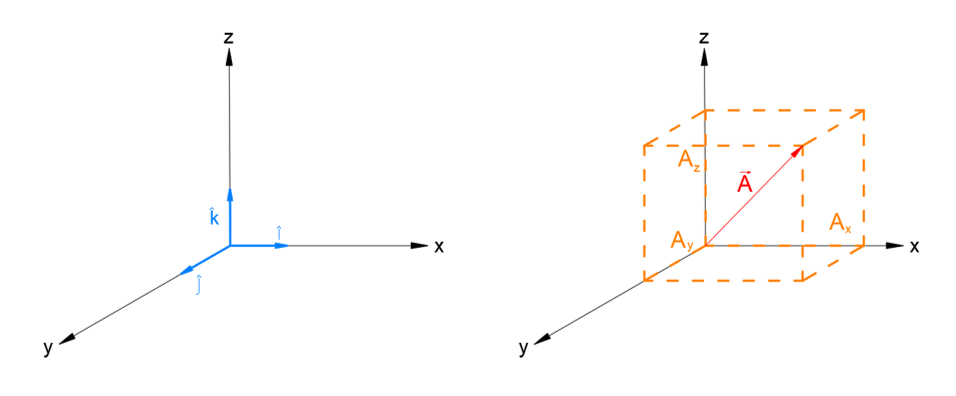
\includegraphics[height=6cm]{Imagenes/vectoreuni.png}
\caption{Representación y suma de vectores}\label{fig:Representacion vectores}
\end{figure}
Además de los vectores también existen los escalares para asignar magnitudes, estos solo poseen magnitud. Los vectores pueden sumarse y restarse, es importante notar que se debe tomar en cuenta la dirección y sentido.\\
El sistema de referencia para ubicar el vector es usualmente el sistema de coordenadas cartesianas, con ejes denotados como $x$, $y$ y $z$. Para mayor facilidad de escritura se asignan vectores unitarios a cada uno de los ejes, siendo $\hat{\imath}$, $\hat{\jmath}$ y $\hat{k}$\\
Ahora denotemos un vetor $\vec{r}\in \mathbb{R}^3$, usando coordenadas cartesianas lo podemos denotar como $\vec{r}=(x,y,z)=x\hat{\imath}+y\hat{\jmath}+z\hat{k}$.\\
Existen operaciones algebraicas posibles con los vectores, estás son:\\
Sea el vector $\vec{A}=(A_x,A_y,A_z)$ y el vector $\vec{B}=(B_x,B_y,B_z)$:
\begin{itemize}
\item Suma de vectores $\vec{A}$ y $\vec{B}$:
$$\vec{A}+\vec{B}=(A_x+B_x)\hat{\imath}+(A_y+B_y)\hat{\jmath}+(A_z+B_z)\hat{k}$$
\item Resta de vectores $\vec{A}$ y $\vec{B}$:
$$\vec{A}-\vec{B}=(A_x-B_x)\hat{\imath}+(A_y-B_y)\hat{\jmath}+(A_z-B_z)\hat{k}$$
\item Mulplicación de un escalar $k$ por un vector $\vec{A}$:
$$k\vec{A}= kA_x \hat{\imath}+kA_y\hat{\jmath}+kA_z\hat{k}$$
\item Producto punto entre vectores $\vec{A}$ y $\vec{B}$:
$$\vec{A} \cdot \vec{B}= A_xB_x+A_yB_y+A_zB_z$$
\item Producto cruz entre vectores $\vec{A}$ y $\vec{B}$:
$$\vec{A} \times \vec{B}= \left| {\begin{array}{ccc}
   \hat{\imath} & \hat{\jmath} & \hat{k} \\
   A_x & A_y & A_z\\
   B_x & B_y & B_z\\
  \end{array} } \right|$$
\end{itemize}
Sea $\Omega$ un espacio abierto en $\mathbb{R}^3$ 
Llamaremos campo vectorial sobre Ω a toda función $$F : Ω ⊆ \mathbb{R}^3\rightarrow\mathbb{R}^3$$
Escribiendo en coordenadas cartesianas esto nos queda:
$$\vec{F}(x,y,z)=\vec{F}_1(x,y,z)\hat{\imath}+\vec{F}_2(x,y,z)\hat{\jmath}+\vec{F}_3(x,y,z)\hat{k}$$
Entonces podríamos definir el campo vectorial como un campo que asocia un vector a cada punto del espacio.
\begin{figure}[H]
\centering
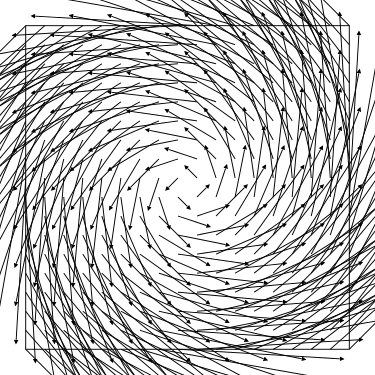
\includegraphics[height=6cm]{Imagenes/campovec.png}
\caption{Campo vectorial. (Fuente: \cite{WikipediaVectorial})}\label{fig:Campo vectorial}
\end{figure}
Para graficar estos campos usualmente se escalan los vectores en cada punto de manera que al mirar el campo completo el dibujo sea entendible, es decir escalamos los vectores para que quepan todos en el dibujo. Otra buena manera de graficar estos campos de forma que sean más fácil de interpretar por parte del lector es coloreando las líneas y establecer una escala de colores para poder interpretar de mejor manera.
\begin{figure}[H]
\centering
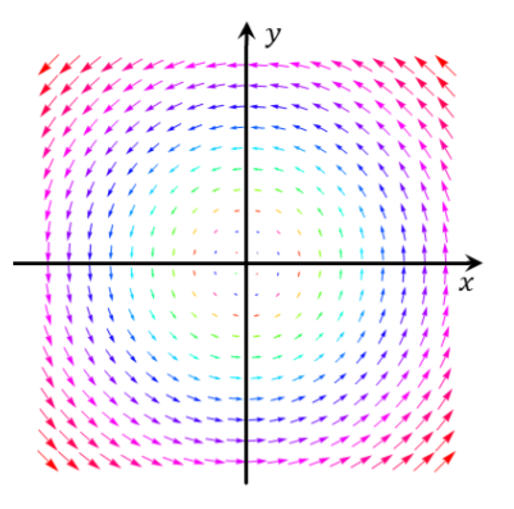
\includegraphics[height=6cm]{Imagenes/campoveccolor.png}
\caption{Campo vectorial. (Fuente: \cite{camposvectoriales})}\label{fig:Campo vectorial en colores}
\end{figure}
Es necesario también saber las operaciones posibles entre campos vectoriales, las fundamentales son 2. El gradiente y el rotacional del campo. Según las definiciones de cite{camposvectoriales2}:
Sea $f:A\subset \mathbb{R}^3\rightarrow \mathbb{R}^3$ un campo vectorial. Suponiendo las condiciones necesarias de derivación definimos divergencia y rotor respectivamente como:
\begin{equation*} 
\mathnormal{div}\;F(x,y,z)=\frac{\partial F_1}{\partial x}(x,y,z)+\frac{\partial F_2}{\partial y}(x,y,z)+\frac{\partial F_3}{\partial z}(x,y,z)
\end{equation*}
\begin{equation*}
\mathnormal{rot}\;F(x,y,z)=\left(\frac{\partial F_3}{\partial y}-\frac{\partial F_2}{\partial z},\frac{\partial F_1}{\partial z}-\frac{\partial F_3}{\partial x},\frac{\partial F_2}{\partial x}-\frac{\partial F_1}{\partial y}\right)=  \left| {\begin{array}{ccc}
   \hat{\imath} & \hat{\jmath} & \hat{k} \\
   \frac{\partial}{\partial x} & \frac{\partial}{\partial y} & \frac{\partial}{\partial z} \\
   F_1 & F_2 & F_3 \\
  \end{array} } \right|
\end{equation*}
Otro tipo de notación también es utilizada, ocupando el simbolo de gradiente como un operador:
$$\nabla = \left(\frac{\partial}{\partial x},\frac{\partial}{\partial y},\frac{\partial}{\partial z}\right)$$
Entonces, reescribimos la divergencia y el rotor utilizando el producto punto y cruz con nuestro operador de la forma:
$$\nabla \cdot F = \left(\frac{\partial}{\partial x},\frac{\partial}{\partial y},\frac{\partial}{\partial z}\right) \cdot \left(F_1,F_2,F_3\right)=\frac{\partial F_1}{\partial x}+\frac{\partial F_2}{\partial y}+\frac{\partial F_3}{\partial z}=\mathnormal{div}\;F$$
$$\nabla \times F = \left| {\begin{array}{ccc}
   \hat{\imath} & \hat{\jmath} & \hat{k} \\
   \frac{\partial}{\partial x} & \frac{\partial}{\partial y} & \frac{\partial}{\partial z} \\
   F_1 & F_2 & F_3 \\
  \end{array} } \right|
  =\left(\frac{\partial F_3}{\partial y}-\frac{\partial F_2}{\partial z},\frac{\partial F_1}{\partial z}-\frac{\partial F_3}{\partial x},\frac{\partial F_2}{\partial x}-\frac{\partial F_1}{\partial y}\right) = \mathnormal{rot}\;F$$
Este operador se puede aplicar sobre si mismo, este 'nuevo' operador se conoce como el 'operador laplaciano' y corresponde a la divergencia del gradiente, para representarlo se utiliza $\Delta$ o $\nabla^2$:
$$\nabla \cdot (\nabla \cdot F) =\nabla^2 \cdot F =\frac{\partial^2 F_1}{\partial x^2}+\frac{\partial^2 F_2}{\partial y^2}+\frac{\partial^2 F_3}{\partial z^2}$$
Existen dos propiedades importantes que debemos tener en cuenta:
\begin{equation}
\label{eq:Rotor de una divergencia}
\nabla \times (\nabla \cdot F)=0
\end{equation}

\begin{equation}
\label{eq:Identidad gradiente}
\nabla \cdot (fV)=f\cdot (\nabla V)-V\cdot\nabla f
\end{equation}
Otro concepto de cálculo vectorial que debemos tener claro son los campos vectoriales conservativos los cuales son de vital importancia en el campo físico. 
Los campos vectoriales que pueden ser definidos bajo el gradiente de una función escalar $f$ son llamados conservativos. Esto es $\vec{F}=\vec{\nabla} f$, además la función escalar $f$ es conocida como la función potencial del campo $\vec{F}$.\\
En otras palabras, esto es, siendo el campo vectorial $\vec{F}(x,y,z)=\vec{F}_1(x,y,z)\hat{\imath}+\vec{F}_2(x,y,z)\hat{\jmath}+\vec{F}_3(x,y,z)\hat{k}$ la función potencial $f(x,y,z)$ del campo $\vec{F}$ está definida como:
$$\frac{\partial f}{\partial x}(x,y,z)=F_1(x,y,z),\qquad \frac{\partial f}{\partial y}(x,y,z)=F_2(x,y,z),\qquad \frac{\partial f}{\partial z}(x,y,z)=F_3(x,y,z)$$
\section{Cálculo integral.}\label{sec:Calculo integral.}
\setcounter{figure}{0}
\setcounter{equation}{0}
En BEM resolveremos ecuaciones diferenciales, en donde a las funciones diferenciales se les aplica muchas veces el concepto de integral. Si bien en este documento no nos adentraremos en demasía en el tema, los teoremas que se presentan a continuación serán de gran utilidad para resolver la problematica planteada:
\begin{itemize}
\item Teorema fundamental del cálculo: Sea $f$ una función escalar.
\begin{equation}
\label{eq:Teorema fundamental del calculo}
\int^b_a \frac{df(x)}{dx}dx=f(b)-f(a)
\end{equation}
\item Teorema fundamental del gradiente: Sea $F$ una función vectorial.
\begin{equation}
\label{eq:Teorema fundamental del gradiente}
\int^b_a \nabla F ds=F(b)-F(a)
\end{equation}
\item Teorema de Gauss:
\begin{equation}
\label{eq:Teorema de Gauss}
\int_\Omega(\nabla\cdot F)d\Omega=\oint_\Gamma n\cdot F d\Gamma
\end{equation}
\item Integración por partes:
\begin{equation}
\label{eq:Integracion por partes}
\int u dv=uv-\int v du
\end{equation}
\end{itemize}
\section{Ecuaciónes Diferenciales.}\label{sec:Ecuaciones Diferenciales.}
En este documento investigaremos el comportamiento de dos ecuaciones de gran importancia en el modelamiento físico de varios fenómenos, por lo que es necesario tener un poco de entendimiento sobre su comportamiento matemático.
\subsection{Ecuación de Laplace.}
Esta es una ecuación de derivadas parciales de tipo elíptico. Es un caso particular de la ecuación de Helmholtz, sin embargo, la ecuación de Laplace junto con la ecuación de Poisson son los dos modelos más simples de las ecuaciones en derivadas parciales (EDP) de tipo elípticas.\\
La ecuación de Laplace en se puede escribir de distintas formas:
Escrita con el operador nabla $\nabla$
\begin{equation}
\nabla^2\phi=0
\end{equation}
Escrita en derivadas, para el caso tridimensional, en coordenadas cartesianas:
\begin{equation}
\frac{\partial^2 \phi}{\partial x^2}+\frac{\partial^2 \phi}{\partial y^2}+\frac{\partial^2 \phi}{\partial z^2}=0
\end{equation}
Esta ecuación es la encargada de modelar el comportamiento de, por ejemplo, el potencial eléctrico en una región sin cargas.
\subsection{Ecuación de Helmholtz.}
Esta ecuación, por otro lado, está compuesta por:
\begin{equation}
(\nabla^2+k^2)\phi=0
\end{equation}